\documentclass[a4paper,12pt]{article} % Tipo de documento y tamaño de letra.
\usepackage[utf8]{inputenc} % Para que reconozca caracteres especiales como tildes.
\usepackage[spanish, es-nodecimaldot]{babel} % Para definir el idioma y el formato de fechas en español.
\usepackage{amsmath, amssymb} % Paquetes para símbolos y ecuaciones avanzadas (Para hacer una ecuación con un recuadro).
\usepackage{ragged2e} % Para justificar textos.
\usepackage{multicol} % Para crear columnas.
\usepackage{slashed} % Para generar números o variables canceladas (Una línea diagonal sobre el número o variable).
\usepackage{graphicx} % Paquete para poner graficas.
\usepackage{float} % Para poder dejar la imagen en un punto fijo del documento.
\usepackage{longtable} % Para tablas largas.
\usepackage{cancel} % Para hacer cancelaciones en medio de operaciones.
\usepackage{xcolor} % Para el color y esas cosas.
\usepackage{apacite} % Paquete para citas APA.
\usepackage{fancyhdr} % Para personalizar encabezados y pies de página.
\usepackage{geometry} % Para ajustar márgenes.
\usepackage{setspace} % Para ajustar el interlineado.
\usepackage{natbib} % Para manejar las citas y que no queden pegadas y feas :P.
\usepackage{hyperref} % Para que los enlaces funcionen con su URL.
\usepackage[version=4]{mhchem}  % Versión recomendada para mayor funcionalidad.
\usepackage{chemfig} %También para hacer estructuras químicas.
\usepackage{array} % Para mejor control de las columnas.
\usepackage{siunitx} % Para unidades físicas.


\pagestyle{fancy}
\fancyhf{} % Limpia encabezados y pies de página predeterminados
\fancyhead[L]{\textbf{DIVULGACIÓN AUDIVISUAL.}} % Encabezado izquierdo
\fancyhead[R]{\textbf{C. CIENTÍFICA.}} % Encabezado derecho
\fancyfoot[C]{\thepage} % Número de página en el centro del pie

\geometry{headheight=12.96115pt, top=1in, bottom=1in, left=1in, right=1in}
\begin{document}


\begin{figure}[H]
	\centering
	
\includegraphics[width=0.8\textwidth]{Unir.jpg}
\end{figure}

\vspace{\baselineskip}

% Ajustamos manualmente todo ;)
\begin{center}
	\textbf{\Large } \\[0.2cm]
	\vspace{\baselineskip}
	\textbf{Beatriz Clemente Fernández.} \\[0.3cm]
    \textbf{Enric Navarro Cuadro.} \\[0.3cm]
    \textbf{Liz Ángel Núñez Torres.} \\[1.5cm]
	\textbf{Grado en Física.} \\[0.6cm]
	\textbf{Universidad Internacional de La Rioja.} \\[0.6cm]
	\textbf{13 de Enero 2026.}
\end{center}


\newpage


\begin{abstract}
\end{abstract}

\begin{justify}
    El descubrimiento, publicado recientemente en la revista \textbf{Nature} sobre la \textbf{actividad eléctrica en la atmosfera} proporciona un nuevo paradigma respecto a lo que sabiamos sobre la superficie de nuestro vecino rojo.
\end{justify}

\begin{justify}
    Hemos recreado un vídeo divulgativo con imagenes  para ejemplificar los estudios y las pruebas recaudadas por el \textbf{Rover Perseverance}.
\end{justify}

\section{Vídeo.}

\vspace{\baselineskip}

\vspace{\baselineskip}

\vspace{\baselineskip}


\begin{figure}[ht]
    \centering
    \href{https://youtu.be/6I02qP7WJDg}{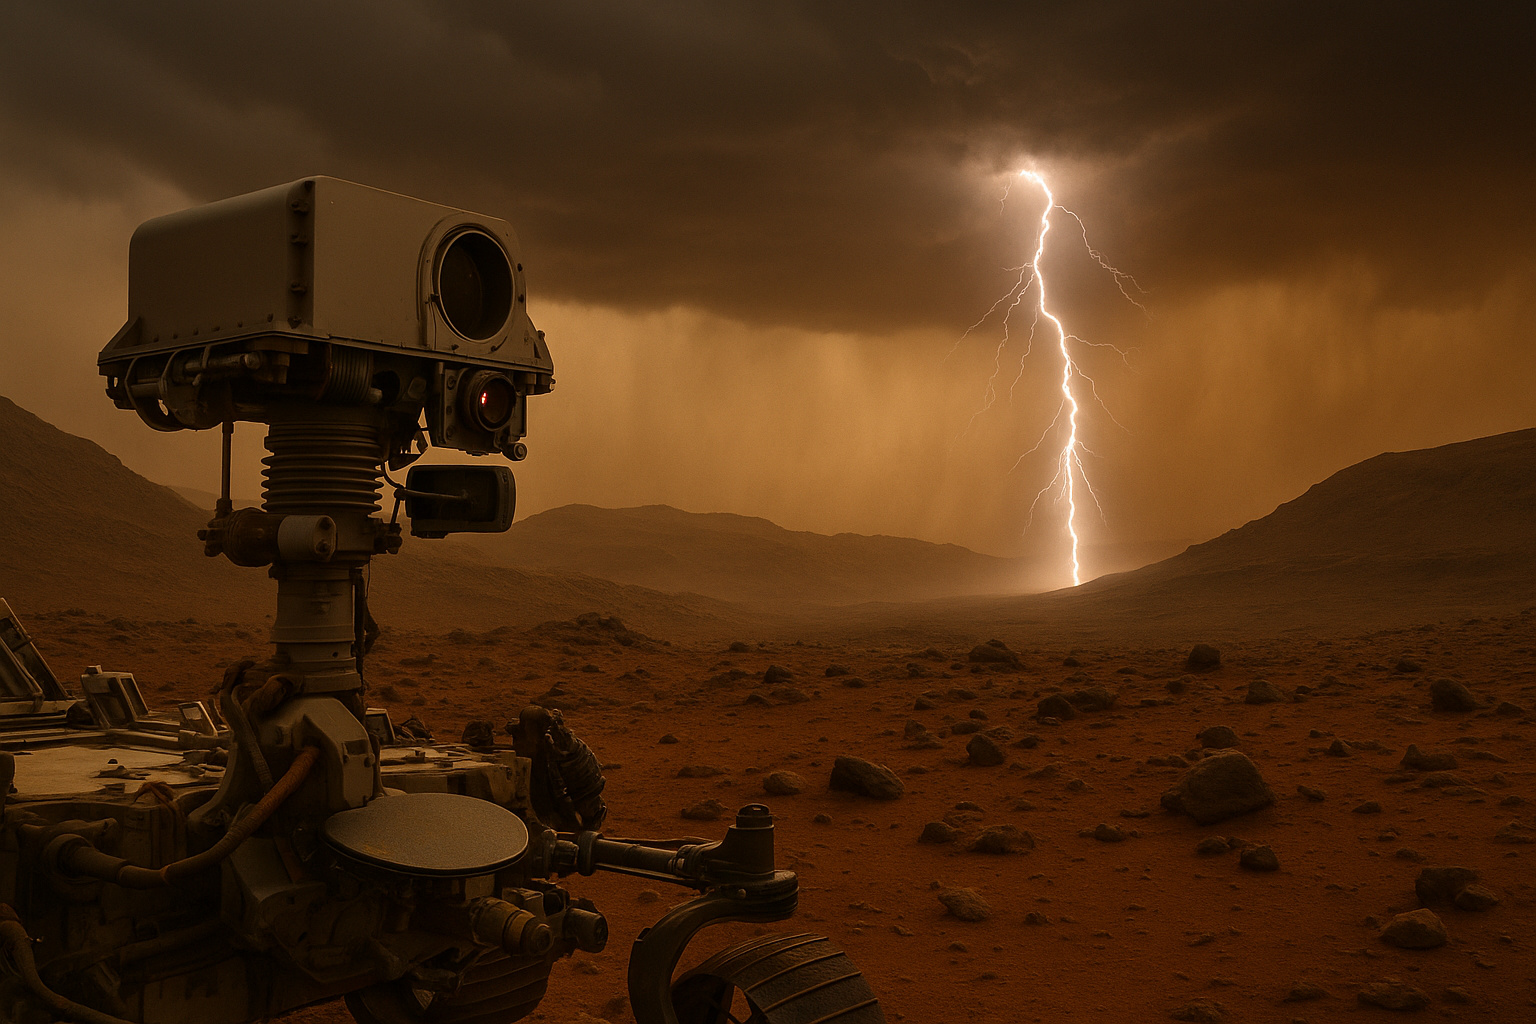
\includegraphics[width=1.0\textwidth]{thunder_mars.jpg}}
    \caption{\href{https://youtu.be/6I02qP7WJDg}{Haz clic aquí o en la imagen para ver el vídeo.}}
    \label{fig:ejemplo}
\end{figure}

\newpage

\setlength{\bibsep}{12pt} % Ajusta la separación entre referencias
\bibliographystyle{apacite} % Estilo APA
\bibliography{citas} % Archivo de referencias
\nocite{*}


\begin{figure}[H]
    \centering
    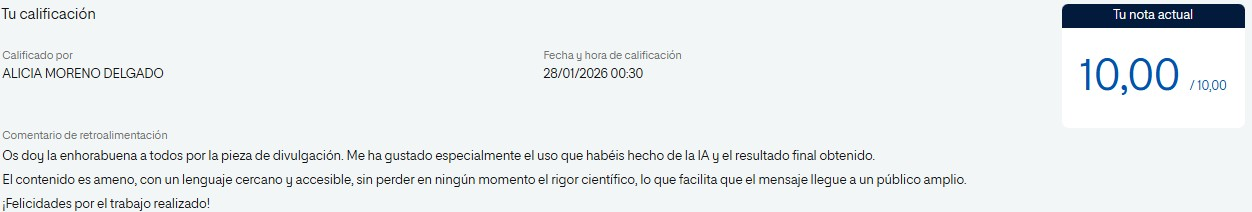
\includegraphics[width=1.1 \textwidth]{calificación.jpg}
\end{figure}






\end{document}